\documentclass[11pt,a4paper]{article}

% --- Encoding & Turkish characters (no babel: math-safe) -------------------
\usepackage[T1]{fontenc}
\usepackage[utf8]{inputenc}
\usepackage{lmodern}

% --- Math / tables / figures ----------------------------------------------
\usepackage{amsmath,amssymb,amsfonts}
\usepackage{booktabs}
\usepackage{graphicx}
\usepackage{algorithm}
\usepackage{algpseudocode}
\usepackage[table]{xcolor}
\usepackage{geometry}
\geometry{margin=2.4cm}
\usepackage{caption}
\usepackage[hidelinks]{hyperref}

\graphicspath{{../results/figures/}{./}}

% kutu: sezgisel açıklamalar için (yalnız xcolor + savebox; ek paket gerekmez)
\newsavebox{\sezgibox}
\newenvironment{sezgi}
  {\begin{lrbox}{\sezgibox}%
   \begin{minipage}{\dimexpr\linewidth-2\fboxsep-2\fboxrule\relax}%
   \small\textbf{\color{blue!55!black}Sezgi.}~}
  {\end{minipage}\end{lrbox}%
   \par\smallskip\noindent
   \fcolorbox{blue!45!black}{blue!5}{\usebox{\sezgibox}}%
   \par\smallskip}

\newcommand{\R}{\mathcal{R}}
\newcommand{\T}{\mathcal{T}}
\newcommand{\Hspatial}{\texttt{H\_SPATIAL}}
\newcommand{\Hcrit}{\texttt{H\_CRIT}}
\newcommand{\Htemp}{\texttt{H\_TEMP}}
\newcommand{\Hstab}{\texttt{H\_STAB}}
\newcommand{\Hrecov}{\texttt{H\_RECOV}}

\title{\textbf{AHE-MRTA: Ekosistem-Güdümlü Paradigma Seçimi}\\[3pt]
\large Yöntemin Sade ve Ayrıntılı Anlatımı}
\author{AHE-MRTA Projesi --- Teknik Doküman}
\date{\today}

\begin{document}
\maketitle

% ==========================================================================
\section*{Özet (bir paragrafta yöntem)}
Birden çok robotu, gelen görevlere atamak istiyoruz. Görevler zaman içinde
çıkıyor, robotlar bazen bozuluyor, bazı görevlerin son teslim zamanı
(deadline) yaklaşıyor. \textbf{Tek bir atama kuralı her duruma uymaz:} en
yakın robotu seçmek yoğunlukta hızlıdır ama deadline'ı kaçırabilir; deadline'a
kilitlenmek arıza anında yavaş kalır; ``kararı bir kez ver, bir daha
değiştirme'' yaklaşımı kararlıdır ama bozulan robotun işini kurtaramaz.
\textbf{AHE-MRTA'nın fikri:} bu kuralları (paradigmaları) bir
\emph{ekosistemde} yarıştırmak ve her an, o anki duruma en uygun kuralı
otomatik seçmek. Robotların ve görevlerin durumu dört sayıya
(\emph{işletim durum vektörü}) sıkıştırılır; bu dört sayı, beş ``hormonun'' (her
biri bir atama kuralı) gücünü günceller; en güçlü hormon o anki kuralı seçer
ve atamayı yapar. Böylece sistem, koşullar değiştikçe kural değiştirir.
Tüm akış Şekil~\ref{fig:diagram}'dedir.

\tableofcontents
\bigskip

% ==========================================================================
\section{Yöntemin Mantığı: Neden ``Ekosistem''?}
\label{sec:overview}

Diyelim ki bir saha ekibini yönetiyorsunuz. Bazen ``en yakın olan gitsin''
dersiniz, bazen ``en acil işi önce bitirelim'', bazen bir araç bozulunca
``onun işlerini hemen başkalarına dağıtalım''. \textbf{Aynı kural her zaman
doğru değildir; doğru kural duruma bağlıdır.} Literatürde buna
\emph{no-free-lunch} denir: hiçbir tek sezgisel (heuristic) tüm koşullarda en
iyi olamaz.

AHE-MRTA tam da bunu yapar: birden çok atama kuralını elinde tutar ve
\textbf{çalışma sırasında} aralarında geçiş yapar. Geçişi bir
\emph{biyomimetik ekosistem} ile yönetir --- doğadaki gibi, koşullara en uygun
``tür'' (burada: atama kuralı) baskın hale gelir. Mekanizmanın üç parçası
vardır:

\begin{enumerate}
  \item \textbf{İşletim Durum Vektörü} $c(t)\in[0,1]^4$ --- ``şu an durum nedir?''
        sorusunun dört sayılık cevabı: ne kadar yoğunuz, kaç robot uygun,
        deadline baskısı var mı, arıza var mı (Bölüm~\ref{sec:context}).
  \item \textbf{Ekosistem dinamiği} $D(t)\in\mathbb{R}^5$ --- beş kuralın
        (hormonun) o anki ``gücünü'' tutan ve işletim durumuna göre güncelleyen bir
        yarış (Bölüm~\ref{sec:dynamics}).
  \item \textbf{Seçici (dispatcher)} --- en güçlü hormona karşılık gelen
        kuralı seçip çalıştırır; acil durumlarda (arıza/deadline) yarışı
        beklemeden doğrudan müdahale eder
        (Bölüm~\ref{sec:dispatch}--\ref{sec:paradigms}).
\end{enumerate}

\begin{sezgi}
Ekosistem \emph{atamayı kendisi çözmez}; sadece ``şu an hangi klasik çözücü
çalışsın?'' sorusunu cevaplar. Bu yüzden yönteme \emph{hiper-sezgisel}
(hyper-heuristic) denir: kuralların üstünde, kural seçen bir katman.
\end{sezgi}

Her kural (paradigma) AHE'nin \emph{kendi} kodudur; rakip bir yönteme iş
devredilmez. Kurallar arası tek ``hafıza'' baskınlık vektörü $D(t)$'dir.

\begin{figure}[t]
  \centering
  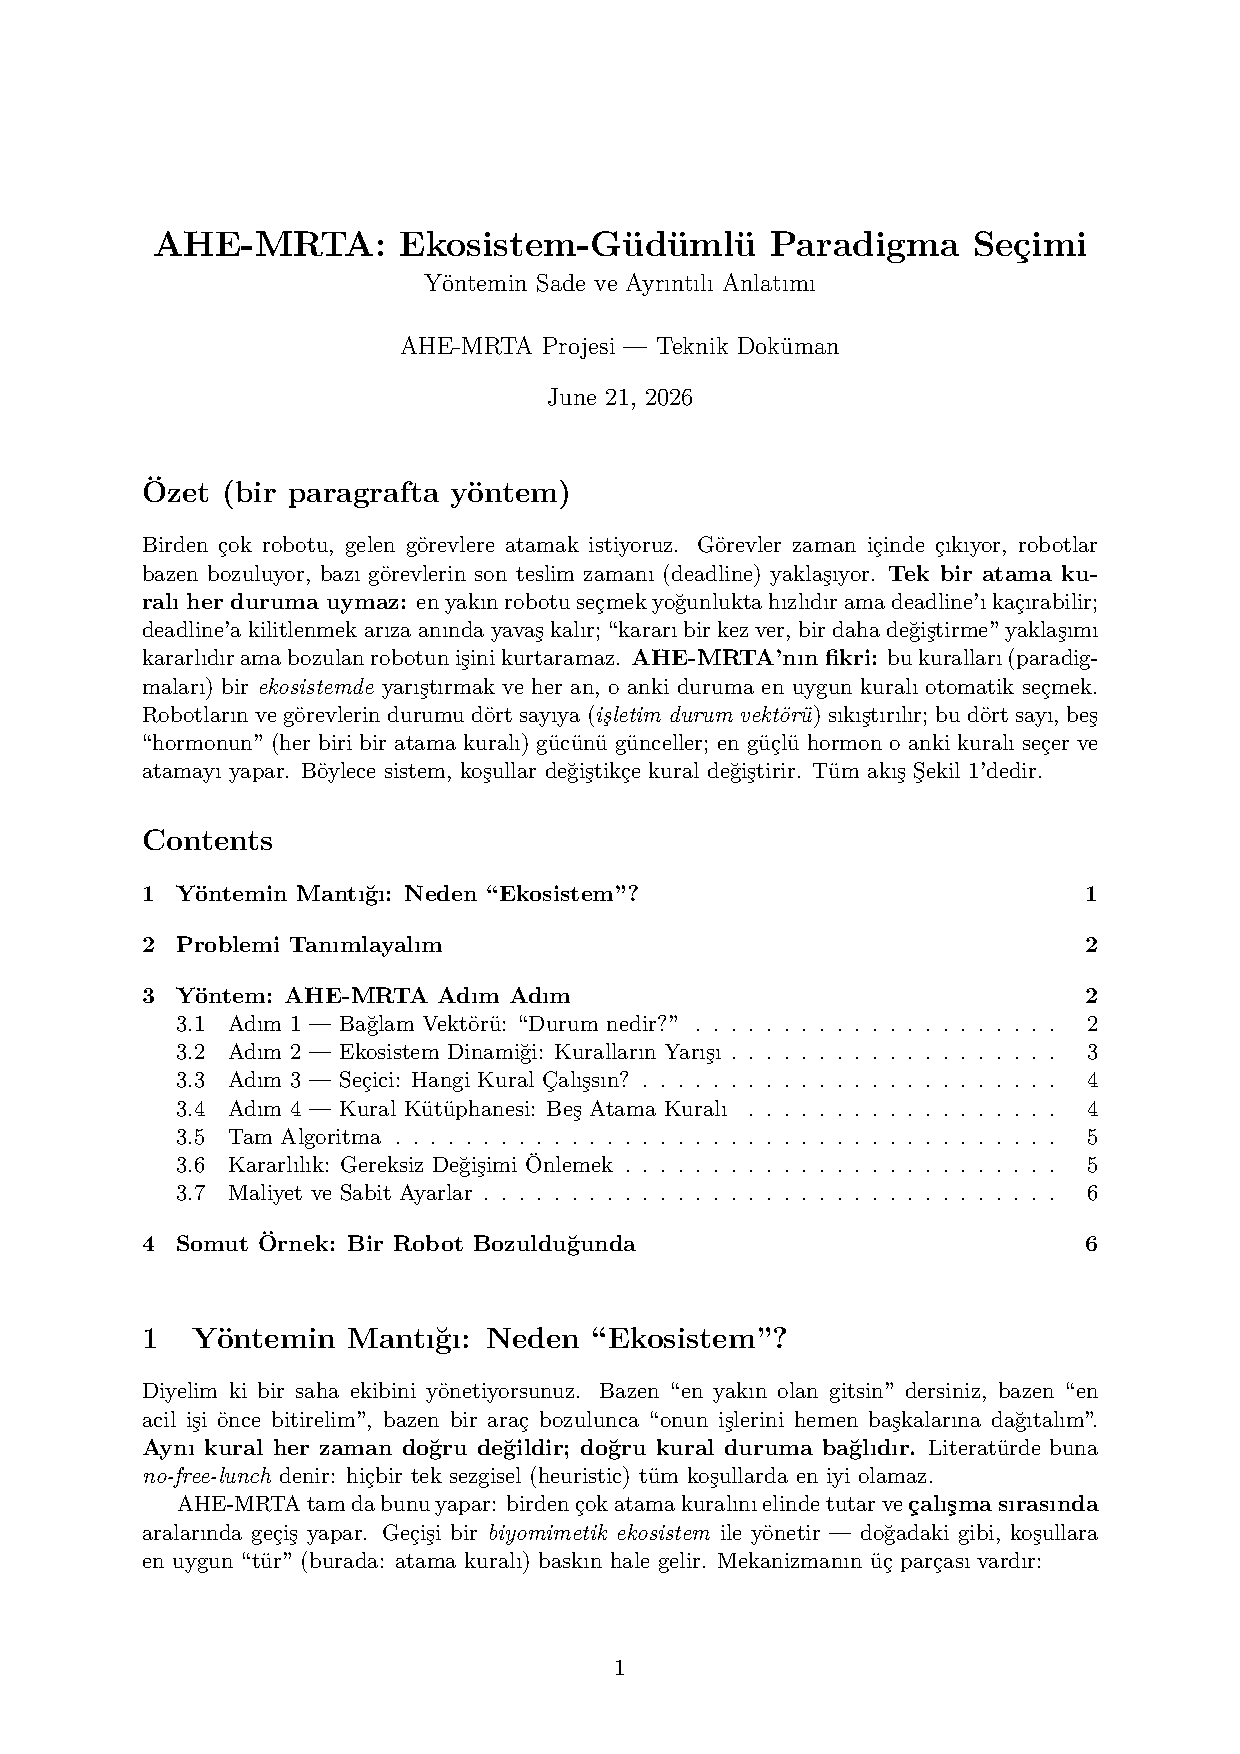
\includegraphics[width=\textwidth]{ahe_method_detailed.png}
  \caption{AHE-MRTA'nın bir karar anındaki (olay) akışı, yukarıdan aşağıya:
  filo ve görev durumu $\rightarrow$ dört sayılık \emph{işletim durum vektörü}
  $\rightarrow$ beş hormonun yarıştığı \emph{ekosistem dinamiği}
  (Denk.~\ref{eq:dominance}) $\rightarrow$ en güçlü hormonun seçilmesi
  ($p^\ast=\arg\max_i D_i$) $\rightarrow$ seçilen kuralın maliyet matrisini
  kurup atamayı (LSA) çözmesi $\rightarrow$ robot-başına görev kuyruklarının
  yayınlanması. Sol kenardaki turuncu döngü, tamamlanan/başarısız görevlerin
  bir sonraki kararda ekosisteme \emph{geri-besleme} olarak dönmesidir.}
  \label{fig:diagram}
\end{figure}

% ==========================================================================
\section{Problemi Tanımlayalım}
\label{sec:problem}

\textbf{Elimizde ne var?} $\R=\{r_1,\dots,r_n\}$ robotlar, $\T(t)$ ise $t$
anında bekleyen (açık) görevler. Her görev $\tau$ şunları taşır: bir konum
$p_\tau$, bir son teslim zamanı (deadline) $d_\tau$, bir öncelik
$\pi_\tau\in\{1,2,3\}$ ve bir yetenek gereksinimi $c_\tau$ (görevi hangi tip
robot yapabilir). Her robot $r$'nin durumu
$s_r(t)=(p_r,\tau_r^{\mathrm{cur}},\phi_r)$: konum, o an yaptığı görev ve
canlı/arızalı bayrağı.

\textbf{Ne karar veriyoruz?} Her \emph{karar anında} $t_k$ (bir görev geldi,
bir robot bozuldu, bir deadline yaklaştı veya periyodik zamanlayıcı ateşledi)
hangi robotun hangi görevi yapacağını söyleyen bir atama
$x_{r,\tau}(t_k)\in\{0,1\}$ üretiriz. İki kısıt: her robotun kuyruğu en fazla
$Q$ görev tutar ($\sum_\tau x_{r,\tau}\le Q$) ve robot, görevin yeteneğini
karşılamalıdır.

\textbf{Bir atama ne kadar ``iyi''?} Her robot--görev çiftine bir
\emph{maliyet} biçeriz; düşük maliyet = iyi eşleşme. Maliyet dört şeyi birleştirir:
yol süresi $T_{r,\tau}$ (uzak robot pahalı), aciliyet
$u_\tau=(d_\tau-t_k)^{-1}$ (deadline yakınsa öne al), kritiklik $\pi_\tau$
(yüksek öncelik önce) ve yeniden-atama cezası $\rho_{r,\tau}$ (gereksiz yere
atamayı değiştirme):
\begin{equation}
  C_{r,\tau} = w_d\,T_{r,\tau} + w_u\,u_\tau^{-1} + w_\pi\,\pi_\tau^{-1}
             + w_\rho\,\rho_{r,\tau}.
  \label{eq:cost}
\end{equation}
Buradaki ağırlıklar $w=(w_d,w_u,w_\pi,w_\rho)$ \textbf{sabit değildir};
o an seçilen kural (paradigma) belirler (Bölüm~\ref{sec:method}). Yani aynı
maliyet formülü, farklı ağırlıklarla farklı ``kişilikler'' kazanır.

\begin{sezgi}
Aciliyet terimi küçük bir incelik taşır: bir görev zaten doğru robotun
kuyruğunda ve zamanında gidecekse, aciliyeti \emph{şişirmeyiz}. Böylece
yaklaşan bir deadline yalnızca \emph{atanmamış} veya risk altındaki görevleri
öne çeker; hâlihazırda yolunda olan atamaları boş yere savurmaz. Bu, gereksiz
atama değişimini (churn) frenler.
\end{sezgi}

\textbf{Neyi ölçüyoruz?} Koşu boyunca dokuz metrik raporlanır: tamamlama oranı
(CR), makespan, ortalama gecikme, deadline ihlal oranı (DVR), arıza kurtarma
süresi, Jain iş-yükü dengesi, yürütme preempt sayısı, yeniden-dağıtım oranı ve
karar gecikmesi. CR ve DVR birincildir.

\begin{sezgi}
\textbf{Dürüst ölçüm kuralı:} Gecikme ve DVR yalnız \emph{tamamlanan}
görevlerden değil, \emph{istenen tüm} görevlerden hesaplanır. Bir yöntem zor
görevleri sessizce bırakırsa, normalde gecikmesi ``yapay olarak'' düşük
görünürdü. Biz bitmeyen görevi ufukta sansürleyip (gecikme) ve deadline ihlali
sayıp (DVR) bu hileyi engelleriz. Bu kural \emph{tüm} yöntemlere aynen
uygulanır.
\end{sezgi}

Son olarak ortam \emph{çevrimiçidir}: görevler akarken, robotlar her an
bozulabilirken, her karar olay başına $50$~ms'lik bir bütçede verilmelidir.

% ==========================================================================
\section{Yöntem: AHE-MRTA Adım Adım}
\label{sec:method}

\subsection{Adım 1 --- İşletim Durum Vektörü: ``Durum nedir?''}
\label{sec:context}

\begin{sezgi}
Sistem karar vermeden önce, o anki durumu \emph{dört sayıya} özetler. Bu dört
sayı, ``hangi kural şu an işe yarar?'' sorusunun ipuçlarıdır.
\end{sezgi}

$n$ robot sayısı, $m$ açık görev sayısı, $\R^{\mathrm{av}}$ uygun robotlar
(canlı, takılı değil, yer var) ve $\R^{\mathrm{f}}$ arızalı/takılı robotlar
olsun. Dört bileşen:
\begin{align}
  c_1 &= \min\!\big(1,\ m/n\big), &&\text{görev yoğunluğu (kaç iş düşüyor)}\\
  c_2 &= |\R^{\mathrm{av}}|/n,    &&\text{robot uygunluğu (eldeki güç)}\\
  c_3 &= \big|\{\tau: d_\tau-t_k\le\Delta_d\}\big|/\max(1,m),
         &&\text{deadline baskısı (acil iş oranı)}\\
  c_4 &= |\R^{\mathrm{f}}|/n,     &&\text{arıza oranı (bozulma)}
\end{align}
deadline ufku $\Delta_d=60$~s. Her sayı $[0,1]$ aralığındadır. Anlamları:
$c_1,c_2$ ``ne kadar yük, ne kadar güç'' dengesini; $c_3$ ``ne kadar acele''
gerektiğini; $c_4$ ``ne kadar bozulma'' olduğunu söyler. Dördü de, robotların
yayınladığı durum özetlerinden hesaplanır --- robotlar arası ekstra iletişim
gerekmez.

Her kuralın (hormonun) bir ``en sevdiği durum'' profili vardır
(Tablo~\ref{tab:proto}). Örneğin arıza kurtarma kuralı (\Hrecov), arıza oranı
(fr) yüksekken parlar; deadline kuralı (\Htemp), deadline baskısı (dp)
yüksekken.

\begin{table}[t]
\centering
\caption{Her kuralın ``en uygun olduğu durum'' profili $V_i\in[0,1]^4$.
Sütunlar: td = görev-yoğunluğu, ra = robot-uygunluğu, dp = deadline-baskısı,
fr = arıza-oranı. Yüksek değer: bu boyut yüksekken kural etkili.}
\label{tab:proto}
\small
\begin{tabular}{@{}lcccc@{}}
\toprule
\textbf{Hormon (kural)} & td & ra & dp & fr \\
\midrule
\Hspatial\ (en yakın)        & 0.7 & 0.7 & 0.1 & 0.1 \\
\Hcrit\ (öncelik önce)       & 0.3 & 0.5 & 0.8 & 0.2 \\
\Htemp\ (deadline, varsayılan)& 0.5 & 0.5 & 0.9 & 0.1 \\
\Hstab\ (kararı koru)        & 0.3 & 0.3 & 0.3 & 0.8 \\
\Hrecov\ (arıza kurtar)      & 0.3 & 0.2 & 0.2 & 0.9 \\
\bottomrule
\end{tabular}
\end{table}

\subsection{Adım 2 --- Ekosistem Dinamiği: Kuralların Yarışı}
\label{sec:dynamics}

\begin{sezgi}
Beş kuralın her birine bir ``güç'' değeri veririz: baskınlık vektörü $D(t)$.
Her karar anında bu güçler güncellenir. Bir kuralın gücü; (a) o anki duruma ne
kadar uyduğuna, (b) son zamanlarda ne kadar iyi iş çıkardığına ve (c)
komşularıyla işbirliği/rekabetine göre artar veya azalır. Doğadaki
\emph{Lotka--Volterra} (avcı-av) rekabeti gibi: uygun olan güçlenir, uygunsuz
olan bastırılır.
\end{sezgi}

Önce \textbf{uyumluluk}: o anki işletim durumu $c$, her kuralın profili $V_i$'ye ne
kadar benziyor? Bunu kosinüs benzerliğiyle ölçeriz:
$v_i(t_k)=\cos(V_i,c(t_k))$ (1'e yakın = çok uygun). Sonra iki seyrek matris
kurallar arası etkileşimi yönetir: \emph{işbirliği matrisi} $A$ (bir kural
güçlenince müttefikini de güçlendirir) ve \emph{baskılama matrisi} $S$ (bir
kural güçlenince rakibini bastırır) --- Tablo~\ref{tab:as}. Güncelleme:
\begin{equation}
\begin{split}
  D(t_{k+1}) &= \mathrm{normalize}\!\Big(\mathrm{clip}_{[0,1]}\!\big(
      \underbrace{\alpha\,D(t_k)}_{\text{hafıza}}
      + \underbrace{\eta\,A\,D(t_k) - \lambda\,S\,D(t_k)}_{\text{işbirliği / baskılama}} \\
      &\qquad + \underbrace{\beta\,\mathbf{p}(t_k)}_{\text{performans}}
      + \underbrace{\gamma\,\mathbf{v}(t_k)}_{\text{uyumluluk}}
      + \underbrace{\delta\,\mathbf{b}(t_k)}_{\text{arıza sıçraması}}
      \big)\Big).
\end{split}
  \label{eq:dominance}
\end{equation}
Terimlerin anlamı, parantezlerde yazıldığı gibi: \textbf{hafıza} ($\alpha=0.85$)
gücün ani sıçramamasını sağlar (geçmişi unutmaz); \textbf{işbirliği/baskılama}
($\eta=\lambda=0.12$) kuralları yarıştırır; \textbf{performans}
$\mathbf{p}=(\mathrm{CR}-\mathrm{FR})\cdot\mathbf{v}$ ($\beta=0.25$) son
zamanlarda işe yarayan kuralı ödüllendirir (tamamlama eksi başarısızlık);
\textbf{uyumluluk} $\mathbf{v}$ ($\gamma=0.20$) duruma uyan kuralı öne çıkarır;
\textbf{arıza sıçraması} $\mathbf{b}$ ($\delta=0.20$) bir robot bozulduğunda
\Hrecov\ ve \Hstab\ kurallarını ani olarak yükseltir. Son adımda
\texttt{normalize} tüm güçleri toplamı $1$ olacak şekilde ölçekler (bir olasılık
dağılımı gibi: $\|D\|_1=1$, $D\ge 0$).

\begin{sezgi}
$\eta AD-\lambda SD$ terimleri bu denklemi bir ``kazanan güçlenir, rakibi
zayıflar'' yarışına çevirir --- bu, çok-robotlu sistemlerde etkili olduğu
gösterilen Lotka--Volterra tipi bir popülasyon dinamiğidir. Sistem atamayı
çözmüyor; \emph{hangi çözücünün} çalışacağını seçiyor.
\end{sezgi}

\begin{table}[t]
\centering
\caption{$A$ (işbirliği) ve $S$ (baskılama) matrislerinin sıfırdan-farklı
girişleri. Diğer tüm girişler sıfır --- yani etkileşim kasıtlı olarak seyrek
ve yorumlanabilir tutulmuştur.}
\label{tab:as}
\small
\begin{tabular}{@{}llll@{}}
\toprule
\textbf{Matris} & \textbf{Kaynak} & \textbf{Hedef} & \textbf{Değer} \\
\midrule
$A$ (işbirliği: güçlendir) & \Hcrit & \Htemp  & 0.20 \\
                           & \Hstab & \Hrecov & 0.20 \\
\midrule
$S$ (baskılama: zayıflat)  & \Htemp & \Hspatial & 0.30 \\
\bottomrule
\end{tabular}
\end{table}

\subsection{Adım 3 --- Seçici: Hangi Kural Çalışsın?}
\label{sec:dispatch}

\begin{sezgi}
Yarışı her zaman beklemek tehlikeli olabilir: bir robot bozulduğunda
``ekosistem yavaşça karar versin'' diye beklersek görevler aksar. Bu yüzden iki
\emph{acil durum kuralı} (sert geçersiz-kılma) vardır; onlar tetiklenmezse
normal yarışın kazananı seçilir.
\end{sezgi}

Seçici sırayla bakar:
\begin{enumerate}
  \item Arıza oranı $c_4>0.05$ ise $\rightarrow$ doğrudan \Hrecov\ (arıza
        kurtarma). Beklemeden.
  \item Deadline baskısı $c_3>0.5$ ise $\rightarrow$ doğrudan \Htemp\
        (deadline kuralı).
  \item İkisi de yoksa $\rightarrow$ yarışın kazananı:
        $p^\ast(t_k)=\arg\max_i D_i(t_k)$.
\end{enumerate}
Eğer güçler birbirine çok yakınsa (belirgin bir kazanan yoksa), varsayılan
olarak \Htemp\ seçilir. Seçilen kural Tablo~\ref{tab:hormones}'teki
mekanizmadır.

\paragraph{İş-koruma ilkesi (work conservation).} Tüm kurallarda ortak bir
altın kural: \textbf{yapılabilir iş varken hiçbir robot boş bırakılmaz.} Her
karar anında her uygun robota o anki kuralın en iyi görevi verilir; bir robot
bozulur veya takılırsa, onun görevleri (öksüzler) yeniden dağıtılır. Böylece
bir aksaklık, \emph{kalıcı görev kaybı} değil, en fazla bir
\emph{yeniden-deneme} maliyeti getirir. Bu, ``kararı bir kez ver'' (commit-once)
yaklaşımının tam tersidir: o yaklaşım, bozulan robotun işlerini koşu bitene
kadar atıl bırakır.

\begin{table}[t]
\centering
\caption{Beş hormon $\rightarrow$ beş atama kuralı.}
\label{tab:hormones}
\small
\begin{tabular}{lll}
\toprule
\textbf{Hormon} & \textbf{Kural (paradigma)} & \textbf{Ne yapar} \\
\midrule
\Hspatial & \texttt{spatial\_greedy} & en yakın uygun robot + uymayanı reddet \\
\Hcrit    & \texttt{priority\_first} & önce yüksek öncelikli görevler \\
\Htemp    & \texttt{edf\_strict}     & en yakın deadline önce (varsayılan) \\
\Hstab    & \texttt{commit\_once}    & kararı koru, değiştirme \\
\Hrecov   & \texttt{orphan\_first}   & önce öksüz görevleri kurtar \\
\bottomrule
\end{tabular}
\end{table}

\subsection{Adım 4 --- Kural Kütüphanesi: Beş Atama Kuralı}
\label{sec:paradigms}

\begin{sezgi}
Beş kural \emph{aynı temel işlemi} kullanır: bir maliyet tablosu kurup en
düşük toplam maliyetli eşleşmeyi bulmak (atama problemi). Farkları, maliyet
tablosunu nasıl şekillendirdikleridir --- yani neye öncelik verdikleri.
\end{sezgi}

Ortak temel: uygunluk-maskeli bir maliyet matrisi $C^{(p)}$ verildiğinde,
kural $p$ şu \emph{doğrusal toplam atama} (LSA, Macar algoritması) problemini
çözer:
\begin{equation}
  x^{(p)} = \arg\min_{x\in\mathcal{X}}
            \sum_{r\in\R}\sum_{\tau\in\T(t_k)} C^{(p)}_{r,\tau}\,x_{r,\tau},
  \label{eq:lsa}
\end{equation}
$\mathcal{X}$ kuralları zorlar: her robot en fazla $Q$ görev
($\sum_\tau x_{r,\tau}\le Q$), her görev en fazla bir robot
($\sum_r x_{r,\tau}\le 1$) ve yetenek uygunluğu. Uygun olmayan çiftlerin
maliyeti $\infty$ yapılır (maskeleme) --- böylece o eşleşme asla seçilmez.
$C_{r,\tau}$ Denk.~\eqref{eq:cost}'nin temel maliyeti olmak üzere, beş kural
şöyle ayrışır:
\begin{itemize}
  \item \textbf{\texttt{spatial\_greedy}} (\Hspatial): Maliyet yalnız yol
        süresidir ($C^{(p)}_{r,\tau}=T_{r,\tau}$). Her görevi en yakın uygun
        robota verir. \emph{Ne zaman iyi:} yoğunlukta, hız önemliyken.
  \item \textbf{\texttt{priority\_first}} (\Hcrit): Görevleri öncelik
        katmanlarına ($3>2>1$) böler ve önce yüksek öncelikli katmanı eşler;
        kritik görevler robotları ilk kapar. \emph{Ne zaman iyi:} kritik
        görevler varken.
  \item \textbf{\texttt{edf\_strict}} (\Htemp, varsayılan): Görevleri en yakın
        deadline'a göre sıralar ve ``zamanında varamayacak'' eşleşmeleri sert
        biçimde eler (varış $>$ deadline $\Rightarrow$ maliyet $\infty$).
        Ardından, deadline'ı bozmadan yolu kısaltan küçük bir
        \emph{ucuz-ekleme} (cheapest-insertion) düzeltmesi uygular. \emph{Ne
        zaman iyi:} deadline baskısı yüksekken (varsayılan kural).
  \item \textbf{\texttt{commit\_once}} (\Hstab): Bir robotun kuyruğundaki görev
        yenilmez bir ``sadakat bonusu'' alır; atamalar dondurulur, gereksiz
        değişim (churn) sıfırlanır. \emph{Ne zaman iyi:} kararlılık kritikken.
  \item \textbf{\texttt{orphan\_first}} (\Hrecov): Bir robot bozulunca/takılınca
        öksüz kalan görevler, herkesten önce özel bir kurtarma turunda atanır.
        \emph{Ne zaman iyi:} arıza anında (kurtarma süresini kısaltır).
\end{itemize}
Kurallar bağımsızdır (geçişte birbirine durum taşımazlar); tek kalıcı hafıza
$D(t)$'dir. LSA en kötü durumda $O(\max(n,m)^3)$'tür; ama denenen ölçeklerde
her karar milisaniye-altı sürer, yani kural seçimi gerçek-zaman bütçesini
zorlamaz.

\subsection{Tam Algoritma}
\label{sec:algo}
\begin{sezgi}
Aşağıdaki döngü her karar anında bir kez çalışır: durumu oku $\rightarrow$
güçleri güncelle $\rightarrow$ kuralı seç $\rightarrow$ atamayı yap
$\rightarrow$ kuyrukları yayınla.
\end{sezgi}

\begin{algorithm}[H]
\caption{AHE-MRTA Karar Döngüsü (her olayda bir kez)}
\label{alg:ahe}
\begin{algorithmic}[1]
\Require robotlar $\R$, açık görevler $\T(t_k)$, güçler $D(t_k)$, sabitler
$A,S,V$, parametreler $\alpha,\eta,\lambda,\beta,\gamma,\delta$
\State $c \gets \textsc{İşletimDurumVektörü}(\R, \T(t_k))$
  \Comment{4 sayı: $c_1$--$c_4$}
\State $\mathbf{v}\gets(\cos(V_i,c))_{i=1}^5$;\;
       $\mathbf{p}\gets(\mathrm{CR}_k-\mathrm{FR}_k)\cdot\mathbf{v}$;\;
       $\mathbf{b}\gets\textsc{ArızaSıçraması}(\R)$
  \Comment{uyumluluk, performans, arıza}
\State $D\gets\mathrm{normalize}(\mathrm{clip}_{[0,1]}(
       \alpha D+\eta AD-\lambda SD+\beta\mathbf{p}+\gamma\mathbf{v}+\delta\mathbf{b}))$
  \Comment{güçleri güncelle}
\State $p^\ast\gets\textsc{AcilDurumKuralı}(c)$ \textbf{varsa, yoksa}
       $\arg\max_i D_i$
  \Comment{kuralı seç}
\State $x\gets \textsc{Kural}_{p^\ast}(\R,\T(t_k))$
  \Comment{atamayı çöz, Tablo~\ref{tab:hormones}}
\State \textbf{yayınla} $x$'ten robot-başına görev kuyrukları
\State \textbf{return} $D, x$
\end{algorithmic}
\end{algorithm}

\subsection{Kararlılık: Gereksiz Değişimi Önlemek}
\label{sec:stability}

\begin{sezgi}
Her karar anında atamaları sıfırdan kurmak, robotları sürekli yön
değiştirmeye iter (gerçek dünyada: Nav2 yolunu iptal et, baştan git --- pahalı).
Bu yüzden yeniden-planlama \emph{minimal-bozulma} ilkesiyle yapılır: önceki plan
korunur, yalnız gerçekten gerekli olduğunda bozulur.
\end{sezgi}

Üç fren çalkantıyı (churn) bastırır:
\begin{itemize}
  \item \textbf{Kapsamlı arıza-sadakati}: Arıza anında sadakat bonusu yalnız
        \emph{öksüz} görevler için kalkar; sağlıklı atamalar yerinde kalır.
  \item \textbf{Yeniden-atama marj kapısı}: Bir görev, ancak yeni robotta
        tahmini varış eskisine göre \emph{en az \%10} iyileşirse taşınır.
        Muaf: öksüzler, kurtarmalar, deadline'ı çok yakın görevler.
  \item \textbf{Deadline-duyarlı önalım (preempt)}: Takılan robotun kuyruğu
        toptan boşaltılmaz; yalnız beklemenin (tahmini $60$~s) deadline'ı
        kaçıracağı görevler öksüz havuzuna düşer.
\end{itemize}
Bu paketin asıl faydası fiziksel (Gazebo/Nav2) yürütmede görülür: her
yeniden-atama bir yol iptali + yeniden katetme demektir. (Sim, yeniden-atamayı
bedelsiz modeller; bu yüzden buradaki kazanç simde görünmez, sahada görünür.)

\subsection{Maliyet ve Sabit Ayarlar}
\label{sec:complexity}

\textbf{Hesaplama maliyeti.} LSA $O(\max(n,m)^3)$'tür; denenen ölçeklerde
karar gecikmesi milisaniye-altı, ek düzeltme (swap-refine, $\le 3$ tur) ihmal
edilebilir. İletişim ayak izi yalnız görev indeksleridir ($\sim 84$~B/kuyruk);
bellek ihmal edilebilir.

\textbf{Tek-sefer ayarlanır, sonra dokunulmaz.} Hormon--kural haritası
(Tablo~\ref{tab:hormones}), $A/S$ matrisleri (Tablo~\ref{tab:as}), profil
tablosu $V$ (Tablo~\ref{tab:proto}) ve tüm sayısal parametreler
($\alpha{=}0.85$, $\eta{=}\lambda{=}0.12$, $\beta{=}0.25$, $\gamma{=}0.20$,
$\delta{=}0.20$, softmax sıcaklığı $T{=}0.3$) \emph{bir kez} belirlenir ve tüm
senaryolarda, tüm ölçeklerde aynen kullanılır. Senaryoya göre ince ayar yok,
öğrenme yok, uyarlanabilir parametre programı yok. \textbf{Bu önemli:} yöntemin
gücü ince ayardan değil, doğru kuralı doğru anda seçmesinden gelir.

% ==========================================================================
\section{Somut Örnek: Bir Robot Bozulduğunda}
\label{sec:example}

\begin{sezgi}
Teoriyi tek bir anla bağlayalım: 5 robottan biri aniden bozuluyor
(\texttt{robot\_failure}). Sistem ne yapar?
\end{sezgi}

\begin{enumerate}
  \item \textbf{Durumu oku.} Arıza oranı $c_4=1/5=0.2$ olur (diğer sayılar
        anlık duruma göre).
  \item \textbf{Güçleri güncelle.} Arıza sıçraması $\mathbf{b}$, kurtarma
        kuralı \Hrecov'un gücünü yükseltir; ayrıca $V_{\Hrecov}$'un arıza
        boyutu $0.9$ olduğundan uyumluluk $\cos(V_{\Hrecov},c)$ de yüksektir.
  \item \textbf{Kuralı seç.} $c_4=0.2>0.05$ acil durum kuralını tetikler:
        \emph{yarışı beklemeden} doğrudan $p^\ast=\Hrecov$.
  \item \textbf{Atamayı yap.} \texttt{orphan\_first}: bozulan robotun öksüz
        görevleri, sağlıklı robotlara özel bir kurtarma turuyla dağıtılır;
        ardından kalan açık görevler için normal deadline-bipartite çalışır.
  \item \textbf{Yayınla.} Yeni kuyruklar yayınlanır; iş-koruma gereği hiçbir
        uygun robot boş kalmaz. Tamamlama sonuçları bir sonraki turda
        performans geri-beslemesini ($\mathbf{p}$) besler.
\end{enumerate}

İşte AHE-MRTA'nın dayanıklılığının özü budur: bir aksaklık kalıcı kayıp değil,
en fazla bir yeniden-denemedir --- ve sistem, bu anı algılayıp otomatik olarak
``kurtarma moduna'' geçer.

\end{document}
